\chapter{Arithmetic and Algebra}

\begin{quote}
As I made my way home, I thought Jem and I would get grown but there
wasn't much else left for us to learn, except possibly algebra.

\hfill---Harper Lee
\end{quote}


\begin{teachingnote}
Here we outline a story with a series of puzzles. We suggest that the
instructor simply present the puzzles (or similar puzzles) and have
the students solve them rather than go through the entire story in class.
\end{teachingnote}


\begin{activitynote}
Activity~\ref{A:SS} complements this section well.  % Shelby and Scotty
\end{activitynote}


\section{Home Base}

Imagine 600 generations past---that's on the order of 10000 years, the
dawn of what we would call civilization. This is a long time ago, well
before the \textit{Epic of Gilgamesh}. Even then people already knew
the need to keep track of numbers. However, they didn't use the
numbers we know and love (that's right, \textit{love}!), they used
tally-marks.\index{tally-marks} Now what if ``a friend'' of yours had
a time machine? What if they traveled through time and space and they
decided to take you back 500 generations? Perhaps you would meet a
nice man named Lothar\footnote{\textit{Lothar of the Hill People} is
  his full name}\index{Lothar of the Hill People} who is trying to
keep track of his goats. He has the following written on a clay
tablet:
\[
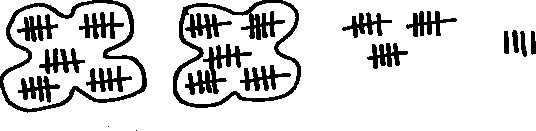
\includegraphics{../graphics/lothar.pdf}
\]
From this picture you discern that Lothar has $69$ goats. Lothar is
studying the tablet intently when his wife, Gertrude, comes in. She
tries in vain to get Lothar to keep track of his goats using another
set of symbols:
\[
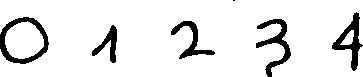
\includegraphics{../graphics/numbers.pdf}
\]
A heated debate between Lothar and Gertrude ensues, the exact details
of which are still a mystery. We do glean the following facts:
\begin{enumerate}
\item Under Gertrude's scheme, five goats are denoted by:
\[

\includegraphics{../graphics/gfive.pdf}
\]
\item The total number of Lothar's goats is denoted by: 
\[
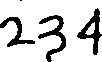
\includegraphics{../graphics/ggoats.pdf}
\]
\end{enumerate}
\begin{question} Can you explain Gertrude's counting scheme?
\end{question}
\QM 

Did I mention that ``your friend's'' time machine is also a spaceship?
Oh\dots Well it is. Now you both travel to the planet Omicron Persei
8.\index{Omicron Persei 8} There are two things you should know about
the inhabitants of Omicron Persei 8:
\begin{enumerate}
\item They only have 3 fingers on each hand.
\item They can eat a human in one bite.
\end{enumerate}
As you can see, there are serious issues that any human visitor to
Omicron Persei 8 must deal with. For one thing, since the Omicronians
only have 3 fingers on each hand, they've only written down the
following symbols for counting:
\[

\includegraphics{../graphics/op8numbers.pdf}
\]
Emperor Lrrr of the Omicronians is tallying how many humans he ate
last week
\[
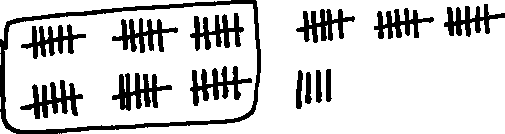
\includegraphics{../graphics/leathuman.pdf}
\]
when his wife, Ndnd, comes in and reminds him that he can write this
number using their fancy symbols as:
\[
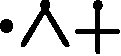
\includegraphics{../graphics/op8numbershe.pdf}
\]
After reading some restaurant menus, you find out that twelve
tally-marks are denoted by the symbols:
\[

\includegraphics{../graphics/op8number12.pdf}
\]
\begin{question} Can you explain the Omicronians' counting scheme?
\end{question}
\QM

At this point you hop back into ``your friend's'' space-time
ship. ``Your friend'' kicks off their shoes. You notice that ``your
friend'' has 6 toes on each foot. You strike up a conversation about
the plethora of toes. Apparently this anomaly has enabled ``your
friend'' to create their own counting scheme, which they say is based
on:
\begin{itemize}
\item Toes
\item Feets
\item Feets of Feets
\item and so on\dots
\end{itemize}
``Your friend'' informs you that they would write the number you know
as ``twenty-six'' as $22$ or ``two feets and two toes.'' What?! Though
you find the conversation to be dull and stinky, you also find out
that ``your friend'' uses two more symbols when they count. ``Your
friend'' uses the letter $A$ to mean what you call ``ten,'' and the
letter $B$ to mean what you call ``eleven!''

\begin{question} Can you explain ``your friend's'' counting scheme?
\end{question}
\QM




%\subsection*{Problems for Section \thesection}\hrule\vspace{1ex}
\begin{problems}
\begin{enumerate}
\item Explain why the following ``joke'' is ``funny:'' \textit{There
  are $10$ types of people in the world. Those who understand base $2$
  and those who don't.}
\item You meet some Tripod aliens, they tally by threes. Thankfully
  for everyone involved, they use the symbols $0$, $1$, and $2$. 
\begin{enumerate}
\item Can you explain how a Tripod would count from $11$ to $201$? Be
  sure to carefully explain what number comes after $22$.
\item What number comes immediately before $10$?  $210$? $20110$?
  Explain your reasoning.
\end{enumerate}
\item You meet some people who tally by sevens. They use the symbols
  $O$, $A$, $B$, $C$, $D$, $E$, and $F$. 
\begin{enumerate}
\item What do the individual symbols $O$, $A$, $B$, $C$, $D$, $E$, and
  $F$ mean?
\item Can you explain how they would count from $DD$ to $AOC$? Be sure
  to carefully explain what number comes after $FF$.
\item What number comes immediately before $AO$?  $ABO$? $HOFFA$?
  Explain your reasoning.
\end{enumerate}
\item Now, suppose that you meet a hermit who tallies by
  thirteens. Explain how he might count. Give some relevant and
  revealing examples.
\item While visiting Mos Eisley spaceport, you stop by Chalmun's
  Cantina. After you sit down, you notice that one of the other aliens
  is holding a discussion on fractions. Much to your surprise, they
  explain that $1/6$ of $30$ is $4$. You are unhappy with this,
  knowing that $1/6$ of $30$ is in fact $5$, yet their audience seems
  to agree with it, not you. Next the alien challenges its audience by
  asking, ``what is $1/4$ of $10$?'' What is the correct answer to
  this question and how many fingers do the aliens have? Explain your
  reasoning.
\item When the first Venusian to visit Earth attended a 6Te grade
  class, it watched the teacher show that
\[
\frac{3}{12} = \frac{1}{4}.
\]
``How strange,'' thought the Venusian. ``On Venus, $\frac{4}{12} =
\frac{1}{4}$.'' What base do Venusians use? Explain your reasoning.
\item When the first Martian to visit Earth attended a high school
  algebra class, it watched the teacher show that the only solution of
  the equation
\[
5x^2-50x+125 = 0
\]
is $x = 5$.

``How strange,'' thought the Martian. ``On Mars, $x = 5$ is a solution
of this equation, but there also is another solution.'' If Martians
have more fingers than humans, how many fingers do Martians have?
Explain your reasoning.

%\begin{teachingnote}
%Here you cannot factor---you must first convert to base $b$.
%\end{teachingnote}

\item In one of your many space-time adventures, you see the equation
\[
\frac{3}{10} + \frac{4}{13} = \frac{21}{20}
\]
written on a napkin. How many fingers did the beast who wrote this
have? Explain your reasoning.
\item What is the smallest number of weights needed to produce every
  integer-valued mass from $0$ grams to say $n$ grams? Explain your
  reasoning.
\item Starting at zero, how high can you count using just your
  fingers?
\begin{enumerate}
\item Explain how to count to $10$.
\item Explain how to count to $35$.
\item Explain how to count to $1023$.
\item Explain how to count to $59048$.
\item Can you count even higher?
\end{enumerate}
Explain your reasoning.
\end{enumerate}

\end{problems}








\section{Arithmetic}\label{S:aritmetic}


Consider this question:

\begin{question}
Can you \textit{think} about something if you lack the
\textit{vocabulary} required to discuss it?
\end{question}
\QM


\begin{activitynote}
Activity~\ref{A:HAr} complements this section well.  % Hieroglyphical Arithmetic
\end{activitynote}


\subsection{Nomenclature}

The numbers and operations we work with have properties whose
importance are so fundamental that we have given them names. Each of
these properties is surely well known to you; however, the importance
of the name is that it gives a keen observer the ability to see and
articulate fundamental structures in arithmetic and algebra.

\paragraph{The Associative Property}\index{associativity} 
An operation \ding{72} is called \textbf{associative} if for all
numbers $a$, $b$, and $c$:
\[
a \,\text{\ding{72}}\, (b \,\text{\ding{72}}\, c) = (a \,\text{\ding{72}}\, b) \,\text{\ding{72}}\, c
\]


\paragraph{The Commutative Property}\index{commutativity}
An operation $\,\text{\ding{72}}\,$ is called \textbf{commutative} if for all
numbers $a$ and $b$:
\[
a \,\text{\ding{72}}\, b = b \,\text{\ding{72}}\, a
\]

\paragraph{The Distributive Property}\index{distributivity}
An operation $\,\text{\ding{72}}\,$ is said to be \textbf{distributive} over another
operation \ding{66} if for all numbers $a$, $b$, and $c$:
\[
a \,\text{\ding{72}}\,(b \,\text{\ding{66}}\, c)  = (a \,\text{\ding{72}}\, b) \,\text{\ding{66}}\, (a\,\text{\ding{72}}\, c)
\qquad\text{and}\qquad (b \,\text{\ding{66}}\, c)\,\text{\ding{72}}\, a  = (b \,\text{\ding{72}}\, a) \,\text{\ding{66}}\, (c\,\text{\ding{72}}\, a)
\]

You may find yourself a bit distressed over some of the notation used
above. In particular you surely notice that we were using crazy
symbols like \ding{72} and \ding{66}. We did this for a reason. The
properties above may hold for more than one operation. Let's explore
this:

\begin{question}
Can you give examples of operations that are associative? Can you give
examples of operations that are not associative?
\end{question}
\QM

\begin{question}
Can you give examples of operations that are commutative? Can you give
examples of operations that are not commutative?
\end{question}
\QM


\begin{question}
Can you give examples of two operations where one distributes over the
other? Can you give examples of operations that do not distribute?
\end{question}
\QM



\subsection{Algorithms}

\begin{teachingnote}
Here we seek to have the students acknowledge the algebra behind many
algorithms. We have given a number of examples illustrating the sort
of work we wish to see.
\end{teachingnote}


\begin{activitynote}
Activities~\ref{A:B1} and~\ref{A:B2} complement  this section well.  % Playing with Blocks & More Playing with Blocks
\end{activitynote}


In elementary school you learned many algorithms. One of the first
algorithms you learned was for adding numbers. Here we show you an
example of the algorithm in action:


\standard{2.NBT.9}


\paragraph{Basic Addition Algorithm}\index{addition algorithm!basic}
Here is an example of the basic addition algorithm:
\[
\begin{tabular}{@{}r@{}}
11~~\\
892\\
+398\\ \hline
1290
\end{tabular}
\]

\begin{question}
Can you describe how to perform this algorithm?
\end{question}

As a gesture of friendship, I'll take this one. All we are doing here
is adding each column of digits at a time, starting with the right-most
digit
\[
\begin{array}[b]{@{}r@{}}
89\textbf{2}\\
+39\textbf{8}\\ \hline
~~\textbf{10}
\end{array}
\qquad
\leadsto
\qquad
\begin{array}[b]{@{}r@{}}
\textbf{1}~~\\
89\textbf{2}\\
+39\textbf{8}\\ \hline
~~~\textbf{0}
\end{array}
\]
If our column of digits sums to $10$ or higher, then we must ``carry''
the tens-digit of our sum to the next column. This process repeats
until we run out of digits on the left.
\[
\begin{array}[b]{@{}r@{}}
\textbf{1}~~\\
8\textbf{9}2\\
+3\textbf{9}8\\ \hline
~\textbf{19}0
\end{array}
\qquad
\leadsto
\qquad
\begin{array}[b]{@{}r@{}}
\textbf{1}1~~\\
\textbf{8}92\\
+\textbf{3}98\\ \hline
\textbf{12}90
\end{array}
\]
We're done!

\begin{question}
Can you show the ``behind-the-scenes'' algebra going on here?
\end{question}

I'll take this one too. Sure, you just write:
\begin{align*}
892 + 398 &= (8\cdot 10^2 + 9\cdot 10 + 2) + (3 \cdot 10^2 + 9\cdot 10 + 8) \\
&= 8\cdot 10^2 + 9\cdot 10 + 2 + 3 \cdot 10^2 + 9\cdot 10 + 8 \\
&= 8\cdot 10^2 + 3 \cdot 10^2 + 9\cdot 10 + 9\cdot 10 + 2 + 8 \\
&= (8 + 3)\cdot 10^2 + (9 + 9)\cdot 10 + (2 + 8) \\
&= (8 + 3)\cdot 10^2 + (9 + 9)\cdot 10 + 10 + 0\\
&= (8 + 3)\cdot 10^2 + (9 + 9+1)\cdot 10 + 0 \\
&= (8 + 3)\cdot 10^2 + (10 + 9)\cdot 10 + 0 \\
&= (8 + 3+1)\cdot 10^2 + 9\cdot 10 + 0 \\
&= 12\cdot 10^2 + 9\cdot 10 + 0 \\
&= 1290
\end{align*}
Wow! That was a lot of algebra. At each step, you should be able to
explain how to get to the next step, and state which algebraic
properties are being used.


\paragraph{Basic Multiplication Algorithm}\index{multiplication algorithm!basic}
Here is an example of the basic multiplication algorithm:

\[
\begin{array}{@{}r@{}}
23~~\\
634\\
\times~~8\\ \hline
5072
\end{array}
\]

\begin{question}
Can you describe how to perform this algorithm?
\end{question}

Me me me me! All we are doing here is multiplying each digit of the
multi-digit number by the single digit number.
\[
\begin{array}[b]{@{}r@{}}
63\textbf{4}\\
\times~~\textbf{8}\\ \hline
~~\textbf{32}
\end{array}
\qquad
\leadsto
\qquad
\begin{array}[b]{@{}r@{}}
\textbf{3}~~\\
63\textbf{4}\\
\times~~\textbf{8}\\ \hline
~~~\textbf{2}
\end{array}
\]
If our product is $10$ or higher, then we must ``carry'' the
tens-digit of our product to the next column. This ``carried'' number
is then added to our new product. This process repeats until we run
out of digits on the left.
\[
\begin{array}[b]{@{}r@{}}
\textbf{3}~~\\
6\textbf{3}4\\
\times~~\textbf{8}\\ \hline
~\textbf{27}2
\end{array}
\qquad
\leadsto
\qquad
\begin{array}[b]{@{}r@{}}
\textbf{2}3~~\\
\textbf{6}34\\
\times~~\textbf{8}\\ \hline
\textbf{50}72
\end{array}
\]
We're done!

\begin{question}
Can you show the ``behind-the-scenes'' algebra going on here?
\end{question}

You betcha! Just write:
\begin{align*}
634 \cdot 8 &= (6\cdot 10^2 + 3\cdot 10 + 4) \cdot 8\\
&= 6\cdot 8\cdot 10^2 + 3\cdot 8\cdot 10 + 4\cdot 8\\
&= 6\cdot 8\cdot 10^2 + 3\cdot 8\cdot 10 + 32 & &\text{(\ding{95})}\\
&= 6\cdot 8\cdot 10^2 + (3\cdot 8 + 3)\cdot 10  + 2 & &\text{(\ding{96})}\\
&= 6\cdot 8\cdot 10^2 + 270  + 2 & &\text{(\ding{100})}\\
&= (6\cdot 8+2)\cdot 10^2 + 7\cdot 10 + 2& &\text{(\ding{98})}\\
&= 50\cdot 10^2 + 7\cdot 10  + 2\\
&= 5\cdot 10^3 + 0\cdot 10^2 + 7\cdot 10  + 2\\
&= 5072
\end{align*}
Ahhhhh! Algebra works. Remember just as before, at each step you
should be able to explain how to get to the next step, and state which
algebraic properties are being used.

\begin{question} 
Can you clearly explain what happened between lines (\ding{95}) and
(\ding{96})? What about between lines (\ding{100}) and
(\ding{98})?
\end{question}
\QM


\paragraph{Long-Division Algorithm With Remainder}\index{division algorithm!long, with remainder}
\index{long division} Once more we meet with this old foe---long
division.  Here is an example:
\[
8\,\begin{array}[b]{@{}r@{}r} 
97 &\, \text{R}1\\ 
\cline{1-1}
\Big)\begin{array}[t]{@{}l@{}} 777\\ 
72 \\ 
\divrule{0}{2}  ~57 \\
 ~56\\
 \divrule{1}{2}
~~1
\end{array}
\end{array}
\]


\begin{question}
Can you describe how to perform this algorithm?
\end{question}

Yes! I'm all about this sort of thing. All we are doing here is single
digit division for each digit of the multi-digit dividend (the number
under the division symbol) by the single digit divisor (the left-most
number). We start by noting that $8$ won't go into $7$, and so we see
how many times $8$ goes into $77$.
\[
\textbf{8}\,\begin{array}[b]{@{}r@{}} 
\textbf{9}~~\\ 
\hline
\Big)\begin{array}[t]{@{}l@{}} \textbf{77}7\\ 
\textbf{72} \\ 
\divrule{0}{2}  ~\textbf{5} \\
\end{array}
\end{array}
\qquad\leftrightsquigarrow\qquad
\begin{minipage}{7ex}
\begin{align*}%\index{Division Theorem!for integers}
n &= d\cdot q + r \\
77 &= 8\cdot 9 + 5
\end{align*}
\end{minipage}
\]
Now we drop the other $7$ down, and see how many times $8$ goes into
$57$.
\[
\textbf{8}\,\begin{array}[b]{@{}r@{}} 
9\textbf{7}~\\ 
\hline
\Big)\begin{array}[t]{@{}l@{}} 777\\ 
72 \\ 
\divrule{0}{2}  ~\textbf{57} \\
 ~\textbf{56}\\
 \divrule{1}{2}
~~\textbf{1}\\
\end{array}
\end{array}
\qquad\leftrightsquigarrow\qquad
\begin{minipage}{7ex}
\begin{align*}
n &= d\cdot q + r \\
57 &= 8\cdot 7 + 1
\end{align*}
\end{minipage}
\]
This process repeats until we run out of digits in the dividend.

\begin{question}
Can you show the ``behind-the-scenes'' algebra going on here?
\end{question}

Of course---but this time things will be a bit different.
\begin{align*}
77 &= 8\cdot 9 + 5 \\
77\cdot 10 &= (8 \cdot 9  + 5 )\cdot 10 \\
77\cdot 10 &= 8 \cdot 9 \cdot 10 + 5 \cdot 10 \\
77\cdot 10 + 7 &= 8 \cdot 9 \cdot 10 + 5 \cdot 10 + 7 \\
777 &= 8 \cdot (9 \cdot 10) + 57 & &\text{(\ding{95})}\\
777 &= 8 \cdot (9 \cdot 10) + (8\cdot 7 + 1) & &\text{(\ding{96})}\\
777 &= 8 \cdot (9 \cdot 10) + 8\cdot 7 + 1 & &\text{(\ding{100})}\\
777 &= 8 \cdot (9 \cdot 10+7) + 1 & &\text{(\ding{98})}\\
777 &= 8 \cdot 97 + 1 
\end{align*}
Looks good to me, but remember: At each step you must be able to
explain how to get to the next step, and state which algebraic
properties are being used.


\begin{question} 
Can you clearly explain what happened between lines (\ding{95}) and
(\ding{96})? What about between lines (\ding{100}) and (\ding{98})?
\end{question}
\QM





\paragraph{Long-Division Algorithm Without Remainder}
\index{division algorithm!without remainder} 
Do you remember that the division algorithm can be done in such a way
that there is no remainder?  Here is an example of the division
algorithm without remainder:
\[
4\,\begin{array}[b]{@{}l@{}} 
~0.75\\
\hline
\Big)\begin{array}[t]{@{}l@{}}\, 3.00\\ 
\,2\;8 \\ 
\divrule{0}{3}  
~\,\;20 \\
 ~\,\;20\\
 \divrule{1}{3} \vspace{-1.4em} \\ 
 \divrule{1}{3}
\end{array}
\end{array}
\]

\begin{question}
Can you describe how to perform this algorithm?
\end{question}

I'm getting a bit tired, but I think I can do this last one. Again,
all we are doing here is single digit division for each digit of the
multi-digit dividend (the number under the division symbol) by the
single digit divisor (the left-most number) adding zeros after the
decimal point as needed. We start by noting that $4$ won't go into
$3$, and so we see how many times $4$ goes into $3.0$. Mathematically
this is the same question; however, by thinking of the $3.0$ as $30$,
we put ourselves into familiar territory. Since
\[
4 \cdot 7 = 30 \qquad \Rightarrow \qquad 4 \cdot 7 \cdot 10^{-1} = 30
\cdot 10^{-1} = 3
\]
this will work as long as we put our $7$ immediately to the right of
the decimal point.
\[
\textbf{4}\,\begin{array}[b]{@{}l@{}} 
~\textbf{0.7}  \\
\hline
\Big)\begin{array}[t]{@{}l@{}} \textbf{3.0}\\ 
\textbf{2\;8} \\ 
\divrule{0}{3}  
~\;\textbf{2}
\end{array}
\end{array}
\qquad\leftrightsquigarrow\qquad
\begin{minipage}{7ex}%\index{Division Theorem!for integers}
\begin{align*}
n &= d\cdot q + r \\ 30 &= 4\cdot 7 + 2
\end{align*}
\end{minipage}
\]
Now we are left with a remainder of $.2$. To take care of this, we
drop another $0$ down and see how many times $4$ goes into $20$. Since
\[
4 \cdot 5 = 20 \qquad \Rightarrow \qquad 4 \cdot 5 \cdot 10^{-2} = 5
\cdot 10^{-2} = 0.05
\]
this will work as long as we put our $5$ two spaces to the right of
the decimal point.

\[
\textbf{4}\,\begin{array}[b]{@{}l@{}} 
~0.7\textbf{5}\\
\hline
\Big)\begin{array}[t]{@{}l@{}} 3.0\textbf{0}\\ 
2\;8 \\ 
\divrule{0}{3}  ~\textbf{\;20} \\
 ~\;\textbf{20}\\
 \divrule{1}{3} \vspace{-1.4em} \\ 
 \divrule{1}{3}
\end{array}
\end{array}
\qquad\leftrightsquigarrow\qquad
\begin{minipage}{7ex}
\begin{align*}
n &= d\cdot q + r \\
20 &= 4\cdot 5 + 0
\end{align*}
\end{minipage}
\]
This process repeats until we obtain a division with no remainder, or
until we see repetition in the digits of the quotient.

\begin{question}
Can you show the ``behind-the-scenes'' algebra going on here?
\end{question}

Let's do it:
\begin{align*}
3 &= 4\cdot 0 + 3 \\
3.0 &= (4 \cdot 7  + 2 )\cdot 10^{-1} \\
3.0 &= 4 \cdot (7\cdot 10^{-1})  + 2 \cdot 10^{-1} \\
3.00 &= 4 \cdot (7\cdot 10^{-1})  + 20 \cdot 10^{-2} \\
3.00 &= 4 \cdot (7\cdot 10^{-1})  + (4\cdot 5) \cdot 10^{-2} & &\text{(\ding{100})}\\
3.00 &= 4 \cdot (7\cdot 10^{-1})  + 4\cdot (5 \cdot 10^{-2}) & &\text{(\ding{98})}\\
3.00 &= 4 \cdot (7\cdot 10^{-1}  + 5 \cdot 10^{-2}) \\
3.00 &= 4 \cdot 0.75 
\end{align*}
Looks good to me, but remember: At each step you must be able to
explain how to get to the next step, and state which algebraic
properties are being used.


\begin{question} 
Can you clearly explain what happened between lines (\ding{100}) and
(\ding{98})?
\end{question}
\QM








\begin{problems}
\begin{enumerate}
\item Explain what it means for an operation \ding{72} to be
  \textit{associative}. Give some relevant and revealing examples.
\item \label{P:MA}Consider the following pictures:
\[
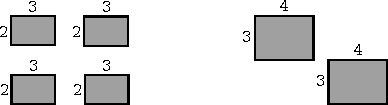
\includegraphics{../graphics/assMult.pdf}
\]
Jesse claims that these pictures represent $(2\cdot 3)\cdot 4$ and
$2\cdot (3\cdot 4)$.
\begin{enumerate}
\item Is Jesse's claim correct? Explain your reasoning.
\item Do Jesse's pictures show the associativity of multiplication? If
  so, explain why. If not, draw new pictures representing $(2\cdot
  3)\cdot 4$ and $2\cdot (3\cdot 4)$ that do show the associativity
  of multiplication.
\end{enumerate}
\item Explain what it means for an operation \ding{72} to be
  \textit{commutative}. Give some relevant and revealing examples.
\item Explain what it means for an operation \ding{72} to \textit{distribute}
  over another operation \ding{66}. Give some relevant and revealing
  examples.
\item Sometimes multiplication is described as \textit{repeated
  addition}. Does this explain why multiplication is commutative? If
  so give the explanation. If not, give another description of
  multiplication that does explain why it is commutative.
\item In a warehouse you obtain $20\%$ discount but you must pay a
  $15\%$ sales tax. Which would save you more money: To have the tax
  calculated first or the discount? Explain your reasoning---be sure
  to use relevant terminology.



\item Money Bags Jon likes to give a tip of $20$\% when he is at
  restaurants. He does this by dividing his bill by $10$ and then
  doubling it. Explain why this works.
\item Regular Reggie likes to give a tip of $15$\% when he is at
  restaurants. He does this by dividing his bill by $10$ and then
  adding half more to this number. Explain why this works.
\item Wacky Wally has a strange way of giving tips when he is at
  restaurants. He does this by rounding his bill up to the nearest
  multiple of $7$ and then taking the quotient (when that new number
  is divided by $7$). Explain why this isn't as wacky as it might
  sound.
%% \begin{teachingnote}
%% The problem above is fundamentally different than the other (related)
%% problems involving tips.
%% \end{teachingnote}

\item Cheap Carl likes to give a tip of $13\frac{1}{3}$\% when he is
  at restaurants. He does this by dividing his bill by $10$ and then
  adding one-third more to this number. Explain why this works.
\item Reasonable Rebbecca likes to give a tip of $18$\% when she is at
  restaurants. She does this by dividing her bill by $5$ and then
  removing one-tenth of this number. Explain why this works.
\item Can you think of and justify any other schemes for computing the
  tip?
\item Here is an example of the basic addition algorithm:
\[
\begin{array}{@{}r@{}}
11~~\\
892\\
+398\\ \hline
1290
\end{array}
\]
\begin{enumerate}
\item Describe how to perform this algorithm.
\item Provide an additional relevant and revealing example
  demonstrating that you understand the algorithm.
\item Show the ``behind-the-scenes'' algebra that is going on here.
\end{enumerate}
\item Here is an example of the column addition
  algorithm:\index{addition algorithm!column}
\[
\begin{array}{@{}r@{}}
892\\
+398\\ \hline
10\\
18~~\\
11~~~\\ \hline
1290
\end{array}
\]
\begin{enumerate}
\item Describe how to perform this algorithm.
\item Provide an additional relevant and revealing example
  demonstrating that you understand the algorithm.
\item Show the ``behind-the-scenes'' algebra that is going on here.
\end{enumerate}

\item If you check out Problems~\ref{P:MS} and \ref{P:DS}, you will
  learn about ``scaffolding'' algorithms.  
\index{addition algorithm!scaffolding}
\begin{enumerate}
\item Develop a scaffolding addition algorithm and describe how to
  perform this algorithm.
\item Provide a relevant and revealing example demonstrating that you
  understand the algorithm.
\item Show the ``behind-the-scenes'' algebra that is going on here.
\end{enumerate}
\item Here is an example of the banker's addition
  algorithm:\index{addition algorithm!banker's}
\[
\begin{array}{@{}r@{}}
892\\
+398\\ \hline
1\textbf{0}\\
1\textbf{9}~~\\
\textbf{12}~~~\\ \hline
1290\,
\end{array}
\]
\begin{enumerate}
\item Describe how to perform this algorithm.
\item Provide an additional relevant and revealing example
  demonstrating that you understand the algorithm.
\item Show the ``behind-the-scenes'' algebra that is going on here.
\end{enumerate}
\item Here is an example of the basic subtraction
  algorithm:\index{subtraction algorithm!basic}
\[
\begin{array}{@{}r@{}r@{}r@{}r@{}}
&   & 8 &  \\
& 8 & \not{\hspace{-.2ex}9} & \hspace{.3ex}\leftexp{1}2\\
- & 3 & 7 & 8\\ \hline
& 5 & 1 & 4
\end{array}
\]
\begin{enumerate}
\item Describe how to perform this algorithm.
\item Provide an additional relevant and revealing example
  demonstrating that you understand the algorithm.
\item Show the ``behind-the-scenes'' algebra that is going on here.
\end{enumerate}
\item Here is an example of the subtraction by addition
  algorithm:\index{subtraction algorithm!by addition}
\[
\begin{array}[c]{@{}r@{}}
892\\
-378\\ \hline
514
\end{array} 
\qquad\leftrightsquigarrow\qquad
\begin{minipage}{40ex}
\begin{align*}
8 + \textbf{4} &= 12 & &\text{add $1$ to $7$ to get $8$} \\
8 + \textbf{1} &= 9 \\
3 + \textbf{5} &= 8
\end{align*}
\end{minipage}
\]
\begin{enumerate}
\item Describe how to perform this algorithm.
\item Provide an additional relevant and revealing example
  demonstrating that you understand the algorithm.
\item Show the ``behind-the-scenes'' algebra that is going on here.
\end{enumerate}


\item Here is an example of the Austrian subtraction
  algorithm:\index{subtraction algorithm!Austrian}
\[
\begin{array}{@{}r@{}r@{}r@{}r@{}}
& 8 & 9 & \hspace{.3ex}\leftexp{1}2\\
- & 3 & \hspace{.3ex}\leftexp{8}{\hspace{-.8ex}\not{\hspace{0ex}7}} & 8\\ \hline
& 5 & 1 & 4
\end{array}
\]
\begin{enumerate}
\item Describe how to perform this algorithm.
\item Provide an additional relevant and revealing example
  demonstrating that you understand the algorithm.
\item Show the ``behind-the-scenes'' algebra that is going on here.
\end{enumerate}

\item If you check out Problems~\ref{P:MS} and \ref{P:DS}, you will
  learn about ``scaffolding'' algorithms.  \index{subtraction algorithm!scaffolding}
\begin{enumerate}
\item Develop a scaffolding subtraction algorithm and describe how to
  perform this algorithm.
\item Provide a relevant and revealing example demonstrating that you
  understand the algorithm.
\item Show the ``behind-the-scenes'' algebra that is going on here.
\end{enumerate}


\item Here is an example of the basic multiplication algorithm:
\[
\begin{array}{@{}r@{}}
23~~\\
634\\
\times~~8\\ \hline
5072
\end{array}
\]
\begin{enumerate}
\item Describe how to perform this algorithm.
\item Provide an additional relevant and revealing example
  demonstrating that you understand the algorithm.
\item Show the ``behind-the-scenes'' algebra that is going on here.
\end{enumerate}
\item\label{P:MS} Here is an example of the scaffolding multiplication
  algorithm: \index{multiplication algorithm!scaffolding}
\[
\begin{array}{@{}r@{}}
634\\
\times~~8\\ \hline
4800\\
240\\
32\\ \hline
5072
\end{array}
\]
\begin{enumerate}
\item Describe how to perform this algorithm.
\item Provide an additional relevant and revealing example
  demonstrating that you understand the algorithm.
\item Show the ``behind-the-scenes'' algebra that is going on here.
\end{enumerate}
\item Here is an example of the basic division algorithm:
\[
8\,\begin{array}[b]{@{}r@{}r} 
97 &\, \text{R}1\\ 
\cline{1-1}
\Big)\begin{array}[t]{@{}l@{}} 777\\ 
72 \\ 
\divrule{0}{2}  ~57 \\
 ~56\\
 \divrule{1}{2}
~~1
\end{array}
\end{array}
\]
\begin{enumerate}
\item Describe how to perform this algorithm.
\item Provide an additional relevant and revealing example
  demonstrating that you understand the algorithm.
\item Show the ``behind-the-scenes'' algebra that is going on here.
\end{enumerate}
\item\label{P:DS} Here is an example of the scaffolding division
  algorithm:\index{division algorithm!scaffolding}
\[
8\,\begin{array}[b]{@{}r@{}} 
7 \\
90\\ 
\hline
\Big)\begin{array}[t]{@{}l@{}} 777\\ 
720 \\ 
\divrule{0}{3}  
~57 \\
 ~56\\
 \divrule{1}{2}
~~1
\end{array}
\end{array}
\]
\begin{enumerate}
\item Describe how to perform this algorithm.
\item Provide an additional relevant and revealing example
  demonstrating that you understand the algorithm.
\item Show the ``behind-the-scenes'' algebra that is going on here.
\end{enumerate}
\item Here is an example of the partial-quotients division
  algorithm:\index{division algorithm!partial-quotients}
\[
8\,\begin{array}[b]{@{}r@{}} 
4\\
10~\\
10~\\
10~\\ 
\hline
\Big)\begin{array}[t]{@{}l@{}} 277\\ 
~80 \\ 
\divrule{0}{3}  
197 \\
~80 \\
\divrule{0}{3}
117 \\
~80 \\
\divrule{0}{3}
~37 \\
~32 \\
\divrule{1}{2}
~~5
\end{array}
\end{array}
\]
\begin{enumerate}
\item Describe how to perform this algorithm---be sure to explain how
  this is different from the scaffolding division algorithm.
\item Provide an additional relevant and revealing example
  demonstrating that you understand the algorithm.
\item Show the ``behind-the-scenes'' algebra that is going on here.
\end{enumerate}
\item Here is an example of the multi-digit multiplication
  algorithm:\index{multiplication algorithm!multi-digit}
\[
\begin{array}{@{}r@{}}
634\\
\times 216\\ \divrule{1}{5}
3804 \\
6340 \\
126800\\ \hline
136944
\end{array}
\]
\begin{enumerate}
\item Describe how to perform this algorithm.
\item Provide an additional relevant and revealing example
  demonstrating that you understand the algorithm.
\item Show the ``behind-the-scenes'' algebra that is going on
  here---you may assume that you already know the algebra behind the
  basic multiplication algorithm.
\end{enumerate}
\item Here is an example of the addition algorithm with decimals:
\[
\begin{array}{@{}r@{}}
1\hspace*{4.2ex}\\
37.2~~\\
+8.74\\ \hline
45.94
\end{array}
\]
\begin{enumerate}
\item Describe how to perform this algorithm.
\item Provide an additional relevant and revealing example
  demonstrating that you understand the algorithm.
\item Show the ``behind-the-scenes'' algebra that is going on here.
\end{enumerate}
\item Here is an example of the multiplication algorithm with
  decimals:
\[
\begin{array}{@{}r@{}}
3.40\\
\times~.21\\ \hline
340\\
6800\\
\hline
.7140
\end{array}
\]
\begin{enumerate}
\item Describe how to perform this algorithm.
\item Provide an additional relevant and revealing example
  demonstrating that you understand the algorithm.
\item Show the ``behind-the-scenes'' algebra that is going on here.
\end{enumerate}
\item Here is an example of the division algorithm without remainder:
\[
4\,\begin{array}[b]{@{}l@{}} 
~0.75\\
\hline
\Big)\begin{array}[t]{@{}l@{}} 3.00\\ 
2\;8 \\ 
\divrule{0}{3}  ~\;20 \\
 ~\;20\\
 \divrule{1}{3} \vspace{-1.4em} \\ 
 \divrule{1}{3}
\end{array}
\end{array}
\]
\begin{enumerate}
\item Describe how to perform this algorithm.
\item Provide an additional relevant and revealing example
  demonstrating that you understand the algorithm.
\item Show the ``behind-the-scenes'' algebra that is going on here.
\end{enumerate}
\item In the following addition problem, every digit has been
  replaced with a letter.
\[
\begin{tabular}{@{}r@{}}
\texttt{MOON}\\
$+$\texttt{ SUN}\\ \hline
\texttt{PLUTO}
\end{tabular}
\]
Recover the original problem and solution. Explain your reasoning.
Hint: $\texttt{S}=6$ and $\texttt{U}=5$.
\item In the following addition problem, every digit has been
  replaced with a letter.
\[
\begin{tabular}{@{}r@{}}
\texttt{SEND}\\
$+$\texttt{MORE}\\ \hline
\texttt{MONEY}
\end{tabular}
\]
Recover the original problem and solution. Explain your reasoning.
\item In the following subtraction problem, every digit has been
  replaced with a letter.
\[
\begin{tabular}{@{}r@{}}
\texttt{DEFER}\\
$-$\texttt{DU7Y}\\ \hline
\texttt{N2G2}
\end{tabular}
\]
Recover the original problem and solution. Explain your reasoning.
\item In the following two subtraction problems, every digit has been
  replaced with a letter.
\[
\begin{tabular}{@{}r@{}}
\texttt{NINE}\\
$-$\texttt{TEN}\\ \hline
\texttt{TWO}
\end{tabular}
\qquad\qquad
\begin{tabular}{@{}r@{}}
\texttt{NINE}\\
$-$\texttt{ONE}\\ \hline
\texttt{ALL}
\end{tabular}
\]
Using both problems simultaneously, recover the original problems and
solutions. Explain your reasoning.
\item In the following multiplication problem, every digit has been
  replaced with a letter.
\[
\begin{tabular}{@{}r@{}}
\texttt{LET}\\
$\times$\texttt{ NO}\\ \hline
\texttt{SOT}\\
\texttt{NOT$~$}\\
\hline
\texttt{FRET}
\end{tabular}
\]
Recover the original problem and solution. Explain your reasoning.

%% \begin{teachingnote}
%% The next two problems may seem tedious, but they are very rewarding
%% for students when they are able to finally solve them. While the
%% student should be encouraged to use a calculator, the solution is not
%% pure ``guess and check'' and there is a lot of reasoning that goes
%% into the solution.
%% \end{teachingnote}

\item The following is a long division problem where every digit
  except 7 was replaced by X.
\settowidth\digitwidth{X}
\def~{\hspace{\digitwidth}}
\[
\text{XX}\,\begin{tabular}[b]{@{}r@{}}
X\,7X \\ \hline
\Big)\begin{tabular}[t]{@{}l@{}}
XXXXX \\
X\,7\,7 \\ \divrule{0}{3}
~X\,7X \\
~X\,7X \\ \divrule{1}{3}
~~~XX\\ 
~~~XX \\ \divrule{3}{2}\vspace{-1.4em} \\ 
 \divrule{3}{2}
\end{tabular}
\end{tabular}
\]
Recover the digits from this long division problem. Explain your
reasoning.
%% \begin{teachingnote}
%% Remind students to use their calculator and that to start,
%% $\mathrm{XX}\cdot \mathrm{X} = \mathrm{X}77$.
%% \end{teachingnote}

\item The following is a long division problem where the digits were
replaced by X except for a single $8$. 

\[
\text{XXX}\,\begin{tabular}[b]{@{}r@{}}
XX8XX \\ \hline
\Big)\begin{tabular}[t]{@{}l@{}}
XXXXXXXX \\
~XXX \\ \divrule{1}{3}
~~XXXX \\
~~~XXX \\ \divrule{3}{3}
~~~~XXXX\\ 
~~~~XXXX \\ \divrule{4}{4}\vspace{-1.4em} \\ 
 \divrule{4}{4}
\end{tabular}
\end{tabular}
\]
Recover the digits from this long division problem. Explain your
reasoning.

\end{enumerate}
\end{problems}







\section{Algebra}



Algebra is when you replace a number with a letter, usually $x$,
right? OK---but you also do things with $x$, like make
\textit{polynomials} out of it.

\subsection{Polynomial Basics}

\begin{activitynote}
Activity~\ref{A:CA} complements this section well.  % Comparative Arithmetic
\end{activitynote}



\begin{question} What's a polynomial? 
\end{question}

I'll take this one:
\begin{definition}\index{polynomial}
A \textbf{polynomial} in the variable $x$ is an expression of the form
\[
a_nx^n + a_{n-1}x^{n-1} + \dots + a_1 x + a_0
\]
where the $a_i$'s are all constants and $n$ is a nonnegative integer.
\end{definition}

\begin{question}
Which of the following are polynomials?
\[
3x^3 - 2x + 1 \qquad \frac{1}{3x^3 - 2x + 1} \qquad 3x^{-3} - 2x^{-1} + 1 \qquad 3x^{1/3} - 2x^{1/6} + 1
\]
\end{question}
\QM


Given two polynomials
\begin{align*}
&a_nx^n + a_{n-1}x^{n-1} + \dots + a_1 x + a_0 \\
&b_mx^m + b_{m-1}x^{m-1} + \dots + b_1 x + b_0
\end{align*}
we treat these polynomials much the same way we treat numbers. Note,
an easy fact is that polynomials are equal if and only if their
coefficients are equal---this may come up again!

\begin{question} Are numbers equal if and only if their digits are equal?
\end{question}
\QM

\begin{teachingnote}
This question is foreshadowing a future discussion of real numbers. The
students will probably suggest that it is true---this is OK. We will
address this point later.
\end{teachingnote}

\begin{question} 
Can you explain how to add two polynomials? Compare and contrast this
procedure to the basic addition algorithm.
\end{question}
\QM

\begin{question} 
Can you explain how to multiply two polynomials? Compare and contrast
this procedure to the basic multiplication algorithm.
\end{question}
\QM



\begin{question} 
Can you explain why someone might say that working with polynomials is
like working in ``base $x$?''
\end{question}
\QM


\subsection{Division and Polynomials}

For some reason you keep on signing up for classes with aloof old
Professor Rufus. When he was asked to teach division of polynomials
with remainders, he merely wrote
\[
d(x)\,\begin{tabular}[b]{@{}r@{} r}
$q(x)$ &\, R\,$r(x)$\\ \cline{1-1}
\Big)\begin{tabular}[t]{@{}l@{}}
\bigstrut[t]$n(x)$ 
\end{tabular}
\end{tabular}
\qquad\text{where}\qquad
\begin{tabular}{l}
$d(x)$ is the divisor \\
$n(x)$ is the dividend \\
$q(x)$ is the quotient \\
$r(x)$ is the remainder
\end{tabular}
\]
and walked out of the room, again! Do you have \textit{d\'{e}j\`{a} vu}?

\begin{question} 
Can you give $3$ much needed examples of polynomial long division with
remainders?
\end{question}
\QM

\begin{question} 
Given polynomials $d(x)$, $n(x)$, $q(x)$, and $r(x)$ how do you know
if they leave us with a correct expression above?
\end{question}
\QM


\begin{question} 
Can you explain how to divide two polynomials? 
%Compare and contrast this procedure to the Division Theorem for
%integers.
\end{question}
\QM

\begin{question} 
Can you do the polynomial long division with remainder?
\end{question}
\QM

Again, this question can be turned into a theorem.

\begin{theorem}[Division Theorem]\index{Division Theorem!for polynomials}
Given any polynomial $n(x)$ and a nonconstant polynomial $d(x)$, there exist unique
polynomials $q(x)$ and $r(x)$ such that
\vspace{1in}
\end{theorem}
\noindent The above space has intentionally been left blank for you to
fill in.
\begin{teachingnote}
Here we want the students to realize that
\[
n(x) = d(x)q(x) + r(x)\qquad\text{where } 0 \le \deg(r(x)) < \deg(d(x)) 
\]
\end{teachingnote}




\begin{problems}
\begin{enumerate}
\item Explain what is meant by a \textit{polynomial} in a variable $x$.
\item Given:
\[
3x^7 -x^5 + x^4 -16x^3 + 27 = a_7 x^7 + a_6x^6 + a_5x^5 + a_4x^4 + a_3x^3 + a_2x^2 + a_1x^1 + a_0
\]
Find $a_0$, $a_1$, $a_2$, $a_3$, $a_4$, $a_5$, $a_6$, $a_7$.
\item Given:
\[
6x^5+a_4 x^4 -x^2 + a_0 = a_5 x^5 - 24 x^4 + a_3 x^3 + a_2 x^2 - 5
\]
Find $a_0$, $a_1$, $a_2$, $a_3$, $a_4$, $a_5$.
\item Is it true that polynomials are equal if and only if their
  coefficients are equal? Explain your reasoning.
\item Is it true that numbers are equal if and only if their digits
  are equal? Explain your reasoning.
\item Explain how to add two polynomials. 
\item Explain how to multiply two polynomials.
\item Here is an example of the polynomial division algorithm:
\[
x^2 + 3x + 1\,\begin{tabular}[b]{@{}r@{}r} 
$x-3$~~&\, R\,$9x+4$\\ 
\cline{1-1}
\Big)\begin{tabular}[t]{@{}l@{}} \bigstrut[t] $x^3 + 0x^2 + x + 1$\\ 
$x^3 + 3x^2 + x$ \\ 
\divrule{0}{11}  
\bigstrut[t]~~~$-3x^2 +0x + 1$\\
~~~$-3x^2-9x -3$\\
\divrule{4}{12}
~~~~~~~~~~$9x + 4$
\end{tabular}
\end{tabular}
\]
\begin{enumerate}
\item Describe how to perform this algorithm.
\item Provide an additional relevant and revealing example
  demonstrating that you understand the algorithm.
\item Show the ``behind-the-scenes'' algebra that is going on here.
\end{enumerate}\index{division algorithm!polynomial}
\item State the \textit{Division Theorem} for polynomials. Give some
  relevant and revealing examples of this theorem in action.
\item Given a polynomial
\[
p(x) = a_nx^n + a_{n-1}x^{n-1} + \dots + a_1 x+ a_0
\]
can you find two numbers $L$ and $U$ such that $L \le p(x) \le U$ for
all $x$? If so, explain why. If not, explain why not.
\item Consider all polynomials of the form
\[
a_nx^n + a_{n-1}x^{n-1} + \dots + a_1 x+ a_0
\]
where the $a_i$'s are integers. If you substitute an integer for $x$
will you always get an integer out? Explain your reasoning.
\item Consider the following polynomial:
\[
p(x) = \frac{x^2}{2}+\frac{x}{2}
\]
Will $p(x)$ always returns an integer when an integer is substituted
for $x$? Explain your reasoning.

\item Fix some integer value for $x$ and consider all polynomials of
  the form
\[
a_nx^n + a_{n-1}x^{n-1} + \dots + a_1 x+ a_0
\]
Where the $a_i$'s are integers greater than or equal to $0$. Which
numbers can be represented by such polynomials? Explain your
reasoning.
\item Find a polynomial 
\[
p(x) = a_nx^n + a_{n-1}x^{n-1} + \dots + a_1 x+ a_0
\]
such that $a_i$'s are integers greater than or equal to $0$ and less
than $2$ such that $p(2) = 35$. Discuss how your answer compares to
the representation of $35$ in base $2$. Explain your reasoning.
\item Find a polynomial 
\[
p(x) = a_nx^n + a_{n-1}x^{n-1} + \dots + a_1 x+ a_0
\]
such that $a_i$'s are integers greater than or equal to $0$ and less
than $7$ such that $p(7) = 200$. Discuss how your answer compares to
the representation of $200$ in base $7$. Explain your reasoning.
\item Find a polynomial 
\[
p(x) = a_nx^n + a_{n-1}x^{n-1} + \dots + a_1 x+ a_0
\]
such that $a_i$'s are integers greater than or equal to $0$ and less
than $10$ such that $p(10) = 18$. Discuss how your answer compares to
the representation of $18$ in base $10$. Explain your reasoning.
\item Find a polynomial 
\[
p(x) = a_nx^n + a_{n-1}x^{n-1} + \dots + a_1 x+ a_0
\]
such that $a_i$'s are integers greater than or equal to $0$ and less
than $15$ such that $p(15) = 201$. Discuss how your answer compares to
the representation of $201$ in base $15$. Explain your reasoning.
\item Fix some integer value for $x$ and consider all polynomials of the form
\[
a_nx^n + a_{n-1}x^{n-1} + \dots + a_1 x+ a_0
\]
Where the $a_i$'s are integers greater than or equal to $0$ and less
than $x$. Which numbers can be represented by such polynomials?
Explain your reasoning. Big hint: Base $x$.
\item Fix some integer value for $x$ and consider all polynomials of
  the form
\[
a_nx^n + a_{n-1}x^{n-1} + \dots + a_1 x+ a_0
\]
Where the $a_i$'s are integers greater than or equal to $0$ and less
than $10$. Which numbers can be represented by such polynomials?
Explain your reasoning.

\item Consider $x^2 + x + 1$. This can be thought of as a ``number'' in
  base $x$. Express this number in base $(x+1)$, that is, find $b_0$, $b_1$, $b_2$ such that 
\[
b_2(x+1)^2 +b_1(x+1) + b_0 = x^2 + x + 1.
\]
Explain your reasoning.

\item Consider $x^2 + 2x + 3$. This can be thought of as a ``number'' in
  base $x$. Express this number in base $(x-1)$, that is, find $b_0$, $b_1$, $b_2$ such that 
\[
b_2(x-1)^2 +b_1(x-1) + b_0 = x^2 + 2x + 3.
\]
Explain your reasoning.

\item Consider $x^3 + 2x + 1$. This can be thought of as a ``number'' in
  base $x$. Express this number in base $(x-1)$, that is, find $b_0$, $b_1$, $b_2,$ $b_3$ such that 
\[
b_3(x-1)^3 + b_2(x-1)^2 +b_1(x-1) + b_0 = x^3 + 2x + 1.
\]
Explain your reasoning.

\item If the polynomial
\[
p(x) = a_nx^n + a_{n-1}x^{n-1} + \cdots + a_1x + a_0
\]
is thought of as a ``number'' in base $x$, describe two different ways
to find the base $(x-1)$ coefficients of $p(x)$.

\end{enumerate}
\end{problems}



